\documentclass{article}
% translate with >> pdflatex -shell-escape <file>

\usepackage{pgfplots}
\pgfplotsset{compat=newest}

\pagestyle{empty}

\begin{document}
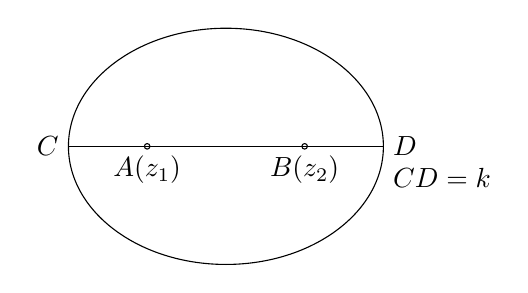
\begin{tikzpicture}%
           \draw (0, 0) ellipse (2 and 1.5);
           \draw (-2, 0) node[anchor=east] {$C$} (2, 0) node[anchor=west]
           {$D$};
           \draw (-2, 0) -- (2, 0);
           \draw (-1, 0) node[anchor=north] {$A(z_1)$} (1, 0)
           node[anchor=north] {$B(z_2)$};
           \draw (-1, 0) circle(1pt) (1, 0) circle(1pt) (2, -.4)
           node[anchor=west] {$CD = k$};
\end{tikzpicture}%
\end{document}

